
In this section, we discuss the performance of the centralized algorithms from Section \ref{sec-3} for a few system configurations. To begin with, we consider a single cell \ac{SISO} model operating at \me{10} dB \ac{SNR} with \me{K = 3} users sharing \me{N = 3} sub-channel resources. The number of packets waiting at the transmitter for each user is given by \me{Q_k = 5,8} and \me{6} bits respectively. 

Fig. \ref{tbl-1} plots the sub-channel wise channel seen by the users followed by the assigned rates over each sub-channel by three different algorithms, \ac{Q-WSRM} allocation, \ac{JSFRA} scheme and the band-wise \ac{Q-WSRM} scheme using \ac{WMMSE} precoder design proposed in \cite{wmmse_shi}. The performance metric used for the comparison of different algorithms is the total number of backlogged bits left over at each slot after the allocation, which is denoted by \me{\chi = \sum_{k = 1}^K \; [ Q_k - t_k ]^+}. It can be seen from Fig. \ref{tbl-1}, that the \ac{Q-WSRM} scheme provides more priority to the third user with \me{Q_{3} = 6} bits compared to the first user with \me{Q_{1} = 5} bits while allocating the first sub-channel. In contrast to the \ac{Q-WSRM} scheme, the \ac{JSFRA} scheme assigns the first user on the first sub-channel thereby reducing the total number of backlogged packets waiting at the transmitter.
%\begin{table*}
%\centering
%\renewcommand{\arraystretch}{1.25} \scriptsize
%\begin{tabular}{|*{14}{c|}}
%\hline
%\multirow{2}{*}{Users} & \multirow{2}{*}{Queued} & \multicolumn{3}{c|}{\multirow{2}{*}{Channel Gains}} & \multicolumn{3}{c|}{Q-WSRM approach} & \multicolumn{3}{c|}{\multirow{2}{*}{JSFRA Scheme}} & \multicolumn{3}{c|}{Q-WSRM band} \\
%\multirow{2}{*}{} & \multirow{2}{*}{Packets} & \multicolumn{3}{c|}{} & \multicolumn{3}{c|}{(\emph{backpreassure} algorithm)} & \multicolumn{3}{c|}{} & \multicolumn{3}{c|}{Alloc Scheme} \\
%\cline{3-14}
% && Sch-\me{1} & Sch-\me{2} & Sch-\me{3} & Sch-\me{1} & Sch-\me{2} & Sch-\me{3} & Sch-\me{1} & Sch-\me{2} & Sch-\me{3} & Sch-\me{1} & Sch-\me{2} & Sch-\me{3} \\
%\hline
%\me{1} & \me{5} & \me{1.71} &  \me{0.53}  &  \me{0.56} & \me{0} &  \me{0}  &  \me{0} & \me{4.91} &  \me{0}  &  \me{0} & \me{0} &  \me{0}  &  \me{0} \\
%\me{2} & \me{8} & \me{0.39} &  \me{1.41}  &  \me{1.03} & \me{0} &  \me{4.46}  &  \me{3.54} & \me{0} &  \me{4.36}  &  \me{0} & \me{0} &  \me{4.39}  &  \me{3.53} \\
%\me{3} & \me{6} & \me{2.34} &  \me{1.26}  &  \me{2.32} & \me{5.72} &  \me{0}  &  \me{0} & \me{0} &  \me{0}  &  \me{5.79} & \me{5.81} &  \me{0}  &  \me{0} \\
%\hline
%\multicolumn{5}{|c|}{Remaining backlogged packets (\me{\chi})} & \multicolumn{3}{c|}{\me{5.28} bits} & \multicolumn{3}{c|}{\me{3.91} bits} & \multicolumn{3}{c|}{\me{5.28} bits} \\
%\hline
%\end{tabular}
%\caption{Sub channel wise allocation for a scheduling instant}
%\label{tbl-1}
%\end{table*}
\begin{figure}
\centering
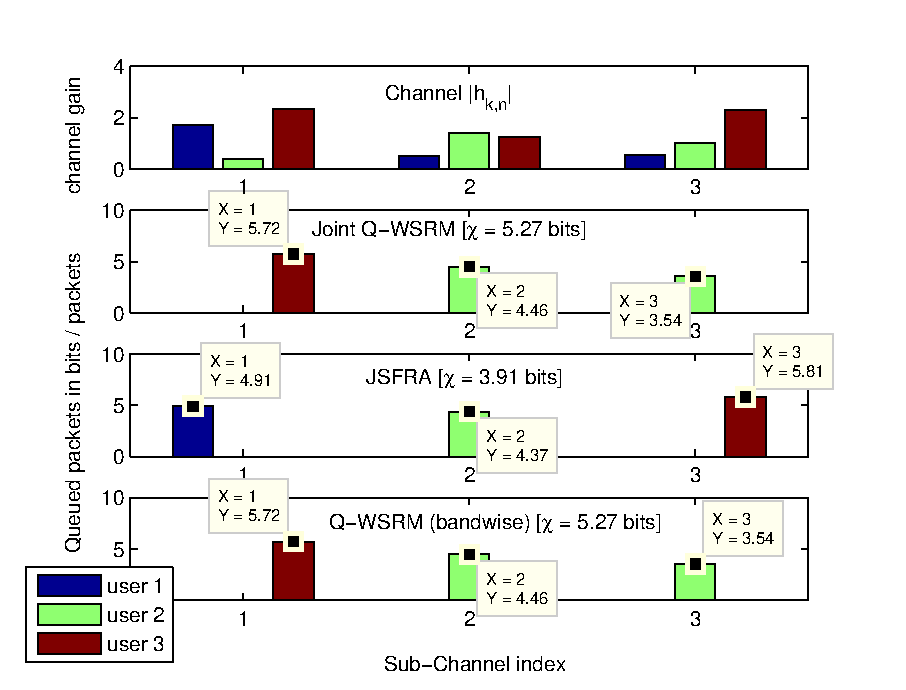
\includegraphics[width=\columnwidth]{tbl-1}
\caption{Allocation for a \ac{SISO} Model comparing different Algorithms}
\label{tbl-1}
\end{figure}

In order to understand the behavior in a \ac{MIMO} framework, we consider a system with \me{N=3} sub-channels and \me{N_B = 3} \acp{BS}, each equipped with \me{N_T = 4} transmit antennas operating at \me{10}dB \ac{SNR}, serving \me{|\mc{U}_b| = 3} users each. The users are located with the maximum interference seen from the neighboring \acp{BS} is limited to \me{-6} dB, thereby simulating a realistic scenario. Fig. \ref{fig-1} shows the performance of the centralized schemes for a single receive antenna system. It compares the total number of \ac{SCA} updates required by the \ac{JSFRA}, \ac{SRA} and the \ac{Q-WSRME} schemes to perform the optimal allocations to minimize the total number of backlogged packets.
\begin{figure*}
\centering
\subfloat[][System \me{\lbrace N,N_B,K,N_T,N_R \rbrace = \lbrace 4,3,9,4,1\rbrace}]{
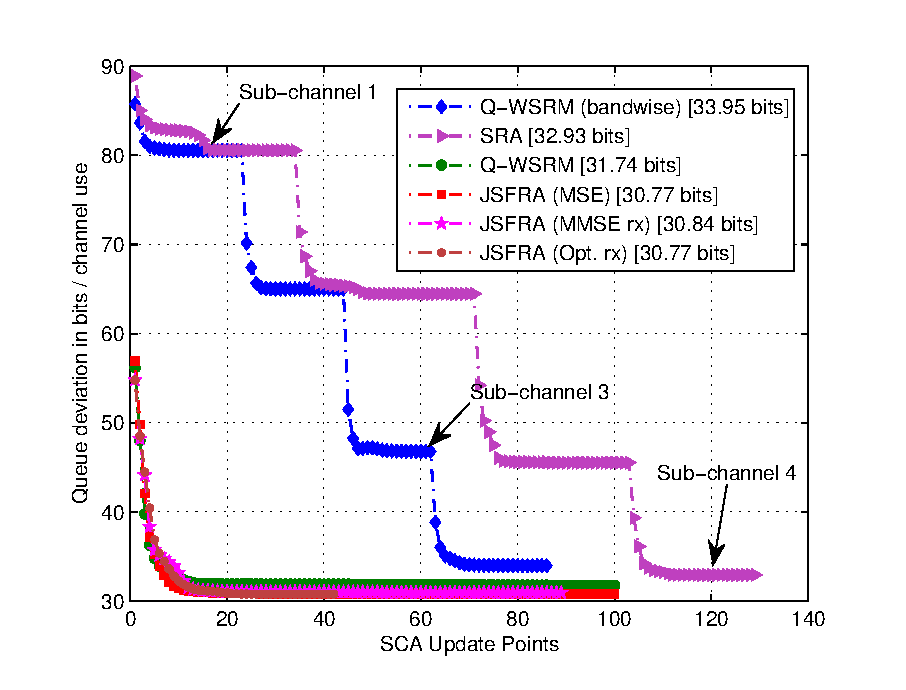
\includegraphics[width=0.48\textwidth]{fig-1-2}
\label{fig-1}}
\hfill
\subfloat[][System \me{\lbrace N,N_B,K,N_T,N_R \rbrace = \lbrace 3,3,9,4,2\rbrace}]{
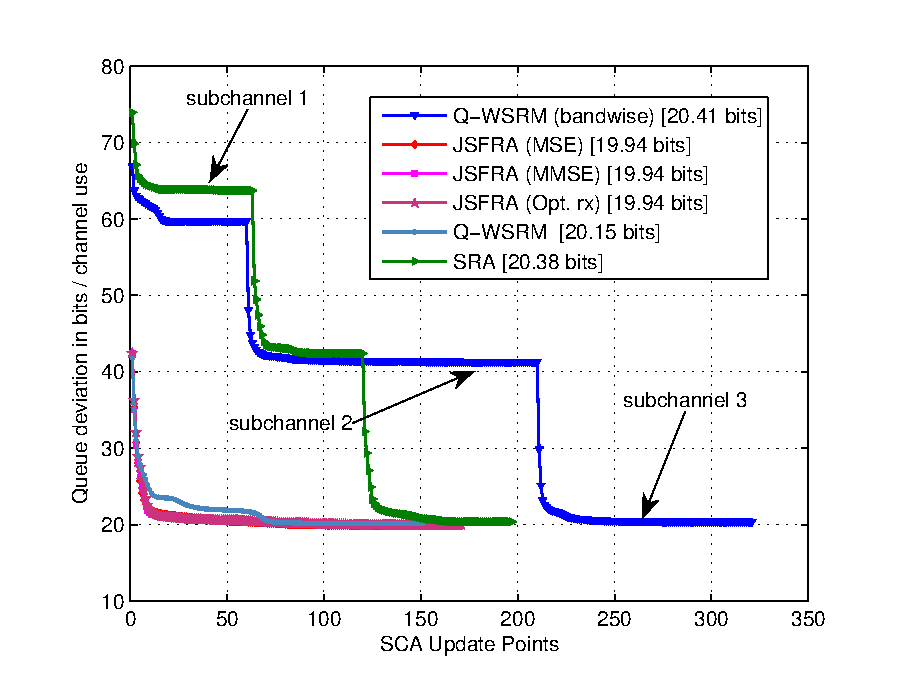
\includegraphics[width=0.48\textwidth]{fig-2-2}
\label{fig-2}}
\caption{Number of backlogged packets at the \ac{SCA} update points}
\label{fig-a}
\end{figure*}

In the sub-channel wise allocations, where the total transmit power is shared equally among the sub-channels, the precoders are designed for each sub-channels independently. In this approach, the precoders are coupled via the number of queued bits which are updated using \eqref{eqn-weight} before designing the precoders for the sub-channels. At each \ac{SCA} points, the number of queued bits are reduced significantly with the introduction of a new sub-channel since the algorithm starts with a random initial point before it converges to an optimal\footnote{due to the nonconvex nature of the original problem} precoders. The total number of backlogged bits at each \ac{SCA} update instant are plotted in Fig. \ref{fig-1} for the discussed centralized schemes and the convergence point are marked with the data tips. Fig. \ref{fig-2} compares the performance of the centralized algorithms for the \me{N_R = 2} receive antennas. In all the schemes, the receive beamformers are updated at the \ac{SCA} update points instead of updating after the \ac{SCA} convergence as in Algorithm. \ref{algo-1}. Since the receiver minimizes the objective for the fixed transmit precoders, the convergence is monotonic as can be seen from the figures.
\begin{table}
\centering
\renewcommand{\arraystretch}{1.25} \scriptsize
\begin{tabular}{|c|*{8}{c}|c|}
\hline
\me{q} & \multicolumn{8}{c|}{user indices} & \me{\chi} \\
\hline
\me{1} & 15.00 & 3.95 & 5.26 & 8.95 & 7.03 & 11.90 & 12.00 & 9.73 & 25.15 \\
\me{2} & 11.23 & 3.93 & 10.76 & 10.65 & 10.27 & 9.68 & 8.77 & 5.90 & 27.77 \\
\me{\infty} & 11.41 & 4.41 & 10.41 & 10.41 & 10.41 & 8.41 &  8.41 &  6.41 & 28.68 \\
\hline
\me{Q_k}  & 15.0 &  8.0 &  14.0 & 14.0 &  14.0 & 12.0 & 12.0 & 10.0  \\
\cline{1-9}
\end{tabular}
\caption{Queue information for the system \me{\lbrace N,N_B,K,N_R \rbrace = \lbrace 5,2,8,1 \rbrace}}
\label{tbl-3}
\end{table}
%\begin{figure}
%\centering
%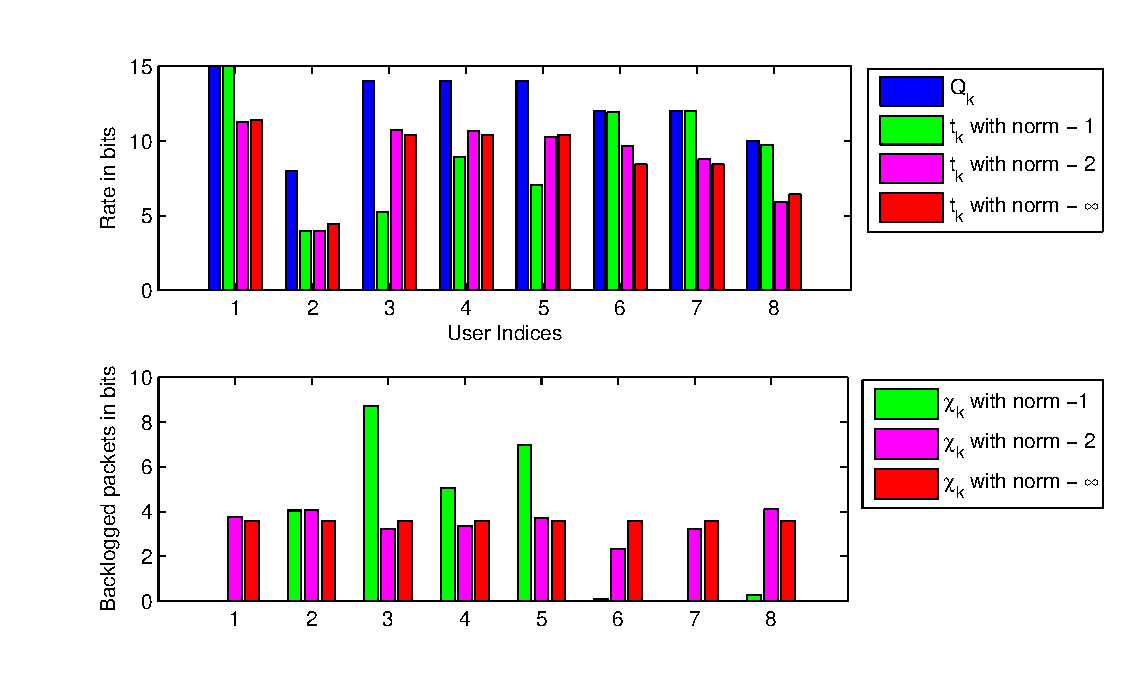
\includegraphics[width=\columnwidth]{tbl-2}
%\caption{Queue information for the system \me{\lbrace N,N_B,K,N_R \rbrace = \lbrace 5,2,8,1 \rbrace}}
%\label{tbl-3}
%\end{figure}

The behavior of the \ac{JSFRA} algorithm for different exponents \me{q} are outlined in the Table. \ref{tbl-3} for the users located at the cell-edge of the system employing \me{N_T = 4} transmit antennas. The configuration is mentioned in the caption of Table. \ref{tbl-3} along with the number of queued bits for each user. It is evident that the algorithm minimizes the queued bits for the \me{\ell_1} norm compared to the \me{\ell_2} norm, which is shown in the column displaying the total number of left over packets \me{\chi} in bits. The \me{\ell_{\infty}} norm provides fair allocation of the resources by making the left over packets to be equal for all users to \me{\chi_k = 3.58} bits. The \me{\ell_{\infty}} norm provides the fair allocation by making the queued deviation equal for all the users after the current allocation irrespective of their channel gains.
